\documentclass[conference]{IEEEtran}
\IEEEoverridecommandlockouts
% The preceding line is only needed to identify funding in the first footnote. If that is unneeded, please comment it out.
% \usepackage{cite}
% Enables Portuguese Brasil
% \usepackage[portuguese]{babel}
%encoding
% Enables code listing
\usepackage{listings}
%--------------------------------------
\usepackage[T1]{fontenc}
\usepackage[utf8]{inputenc}
%--------------------------------------
%Enables the use of greek letter without a math context
\usepackage{textgreek}
%--------------------------------------
%Enables hiperlinks
\usepackage[hidelinks]{hyperref}
%--------------------------------------

\usepackage{amsmath,amssymb,amsfonts}
\usepackage{algorithmic}
\usepackage{graphicx}
\usepackage{textcomp}
\usepackage{xcolor}

\usepackage{color, colortbl}

% The code style
\usepackage{color}
\definecolor{codegreen}{rgb}{0,0.6,0}
\definecolor{codegray}{rgb}{0.5,0.5,0.5}
\definecolor{codepurple}{rgb}{0.58,0,0.82}
\definecolor{backcolour}{rgb}{0.95,0.95,0.92}

\lstdefinestyle{mystyle}{
	backgroundcolor=\color{backcolour},   
	commentstyle=\color{codegreen},
	keywordstyle=\color{magenta},
	numberstyle=\tiny\color{codegray},
	stringstyle=\color{codepurple},
	basicstyle=\footnotesize,
	breakatwhitespace=false,         
	breaklines=true,                 
	captionpos=b,                    
	keepspaces=true,                 
	numbers=left,                    
	numbersep=2pt,                  
	showspaces=false,                
	showstringspaces=false,
	showtabs=false,                  
	tabsize=2
}
\lstset{style=mystyle}
%---------------------------------------

\def\BibTeX{{\rm B\kern-.05em{\sc i\kern-.025em b}\kern-.08em
		T\kern-.1667em\lower.7ex\hbox{E}\kern-.125emX}}

\begin{document}
	\title{A brief review of Quantum Mechanics for Computer Scientists}
	\author{André Furlan - UNESP - Universidade Estadual Paulista "Júlio de Mesquita Filho"}
	\date{2023-06-01}
	\maketitle
	
	\begin{abstract}
		Quantum computers are one of the most promising technologies currently. However, a lack of understanding of its basic concepts may hinder even experienced computer scientists from exploring its possibilities. This document aims to provide a brief review of these concepts to enable those interested in quantum computation to understand and utilize its ideas effectively.
	\end{abstract}
	
	\begin{IEEEkeywords}
		quantum mechanics, quantum computation, qubit
	\end{IEEEkeywords}
	
	\section{Introduction}
		\par In the same century that classical computers, with their classical bits that can only assume one of two values (0 or 1), emerged, another field of knowledge arose: Quantum Mechanics. This field was developed to explain phenomena in the microscopic domain that could not be adequately described by Newtonian mechanics. As some quantum phenomena, such as entanglement and superposition, exhibit counterintuitive behavior, scientists began exploring the possibility of utilizing these behaviors in computing, leading to the birth of quantum computing.
		
	\section{Quantum states}
		\par In quantum mechanics, a \textbf{state} refers to a mathematical representation that provides information about the properties of a physical system. It encapsulates the essential characteristics and behavior of the system, such as its observable quantities and their possible values.\newline
		
		\par The state of a quantum system is described using a formalism called \textbf{state vectors}, which belong to a \textbf{vector space} (more on this in section \ref{sec:vectorspace}) associated with the system. These vectors are often denoted using the "ket" notation (section \ref{sec:ketNotation}), introduced by physicist Paul Dirac, where a state vector is represented as $|\psi\rangle$, pronounced as "ket psi".\newline
		
		\par The state vector represents the system's quantum state, encoding both the information about the system's observable quantities and the probabilities of obtaining specific outcomes upon measurement. The state vector can evolve over time according to the laws of quantum mechanics, capturing the dynamics and changes in the system as it interacts with its environment.\newline
		
		\par A quantum state can be in a \textbf{superposition}, meaning it is not limited to a single definite value but rather exists as a combination of multiple possible states. This superposition arises due to the fundamental principle of quantum mechanics known as \textbf{superposition principle}, which allows states to be in a coherent linear combination of basis states.\newline
		
		\par It is important to note that a state is not a physical object itself, but rather a mathematical representation that provides a comprehensive description of the system's properties.
	
	\section{Complex vector space}
		\label{sec:vectorspace}
		\par A \textbf{vector space} ($V$) over the complex numbers $\mathbb{C}$ is a mathematical structure that allows for the representation of its elements (vectors) and adheres to the following set of rules:
		
		\begin{itemize}
			\item $\alpha \in \mathbb{C}, \alpha . |V_1\rangle \in V$
			\item $\vec{0} , \vec{0} + |V_1\rangle = |V_1\rangle$ (null vector)
			\item $|V_1\rangle + |V_2\rangle = |V_2\rangle + |V_1\rangle$ (commutative)
			\item $|V_1\rangle \in V, |V_2\rangle \in V \implies |V_1\rangle + |V_2\rangle \in V$
			\item $|-V_1\rangle; |V_1\rangle + |-V_1\rangle=\vec{0}, |-V_1\rangle=-|V_1\rangle$ 
			\item $|V_1\rangle + (|V_2\rangle + |V_3\rangle) = (|V_1\rangle + |V_2\rangle) + |V_3\rangle$ (associative)
			\item $\alpha,\beta \in \mathbb{C}; \alpha (|V_1\rangle + \beta . |V_2\rangle) = \alpha . |V_1\rangle + \alpha . \beta . |V_2\rangle $ (distributive)
		\end{itemize}

		\par It is important to highlight that when using the "BraKet" notation described in section \ref{sec:DiracNotation}, the \textbf{basis}, which are \textbf{normalized and mutually orthogonal} vectors within the vector space, is used in combination with other parameters to represent a specific state of interest.\newline
		
		\par In quantum mechanics these \textbf{basis vectors} are called \textbf{system possible states}.
	
	\section{Dirac notation}
		\label{sec:DiracNotation}
			
		\par In quantum mechanics, it is crucial to define the \textbf{range} of values that a particle's state can assume. This concept that will be discussed deeply in section \ref{sec:probAmpli} is known as \textbf{probability amplitude} and it employs two notations: the "ket" and the "bra". These notations are commonly referred to as the \textbf{Dirac's "BraKet" notation}.

		\subsection{Ket notation}
			\label{sec:ketNotation}
			\par The combination of symbols $|$ and $\rangle$ with a value inside is referred to as a "ket." An example is demonstrated in Equation \ref{eq:ketNotationVector}.
			
			\begin{equation}
				|K\rangle = \vec{K} = \{a, b, c, d\}
				\label{eq:ketNotationVector}
			\end{equation}
			
			\par Where $a, b, c, d \in \mathbb{Q}$ and are components of the vector $K$.\newline

			\par In order to describe the state of a particle using the \textbf{vector space basis}, the particle's state can be written using the equation \ref{eq:ketNotationGeneric}.
			
			\begin{equation}
				| \psi \rangle = \alpha . | V_1 \rangle + \beta . | V_2 \rangle
				\label{eq:ketNotationGeneric}
			\end{equation}
		
			\par With $\alpha, \beta$ and $\gamma$ known as \textbf{probability amplitudes}.\newline
						
			\par Simply put, the equation \ref{eq:ketNotationGeneric} and its respective plot depicted in figure \ref{fig:diracPlot} can be interpreted as follows: \textit{The state of $\psi$ within the vector space defined by vectors $V_1$ and $V_2$ is a linear combination ($\alpha$ times vector $V_1$ plus $\beta$ times vector $V_2$)}.
			
			\begin{figure}[h]
				\centering
				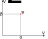
\includegraphics{images/diracPlot}
				\caption{Visual representation of Equation \ref{eq:ketNotationGeneric}. Vectors $V_1$ and $V_2$ must be orthogonal and normalized.}
				\label{fig:diracPlot}
			\end{figure}
	
			\par In quantum mechanics, a state can be represented by different levels depending on the system. For instance, the previous example illustrated a representation of a \textbf{two-level state system}. However, it is important to note that a state can be extended to include one, two, or even multiple levels ($n$).\newline
			
			\par To represent multiple-level states, a common approach is to utilize a vector space with a basis that corresponds to the distinct levels of the system. Each level is associated with a specific vector in the vector space.\newline
			
			\par For instance, consider a three-level system. We can define a basis as ${|V_0\rangle, |V_1\rangle, |V_2\rangle}$, where $|V_0\rangle$, $|V_1\rangle$, and $|V_2\rangle$ represent the vectors associated with the respective levels.
			
			\par In general, a state in a multiple-level system can be expressed as a linear combination of these basis vectors:
			
			\begin{equation}
				|\psi\rangle = \alpha |V_0\rangle + \beta |V_1\rangle + \gamma |V_2\rangle \qquad,
				\label{eq:multipleLevelState}
			\end{equation}
		
			\par Here, $\alpha$, $\beta$, and $\gamma$ are complex coefficients that determine the \textbf{amplitudes} of the state in each level.\newline
			
			\par Being $N=$ the number of levels and $a \in (\alpha, \beta, \gamma, ... , \omega)$ sometimes the equation \ref{eq:multipleLevelState} can be represented as a sum:
			
			\begin{equation}
				|\psi\rangle = \sum_{i=1}^{N} a_i . |V_i\rangle = 
				\begin{bmatrix}
					a_{1} \\
					a_{2} \\
					\vdots \\
					a_{n}
				\end{bmatrix}
				\label{eq:multipleLevelStateSum}
			\end{equation}
		
			\par Some authors prefers to use $|0\rangle, |1\rangle, |2\rangle, \dots , |n\rangle / n < N$ instead of $|V_0\rangle,|V_1\rangle, \dots, |V_n\rangle / n < N$.\newline

			\par Note that this representation is nothing more than another way of defining a \textbf{vector} considering a \textbf{vector space basis} already used in linear algebra, as shown in Equation \ref{eq:linearCombination}!\newline
			
			\begin{equation}
				\label{eq:linearCombination}
				\begin{aligned}
					|\psi\rangle =
					\begin{bmatrix}
						a_{1} \\
						a_{2} \\
						\vdots \\
						a_{n}
					\end{bmatrix} =
					a_1 . \begin{bmatrix}
						1\\
						0\\
						\vdots \\
						0
					\end{bmatrix}+
					a_2 . \begin{bmatrix}
						0\\
						1\\
						\vdots \\
						0
					\end{bmatrix}+
					\dots + a_n . \begin{bmatrix}
						0\\
						0\\
						\vdots \\
						1
					\end{bmatrix}
				\end{aligned}
			\end{equation}
		
			\par Remember this basis vectors $
			\begin{bmatrix}
				1\\
				0\\
				\vdots \\
				0
			\end{bmatrix}, 
			\begin{bmatrix}
				0\\
				1\\
				\vdots \\
				0
			\end{bmatrix}, \dots,
			\begin{bmatrix}
				0\\
				0\\
				\vdots \\
				1
			\end{bmatrix}$ are the \textbf{system possible states}!
		
		\subsection{Probability amplitude}
			\label{sec:probAmpli}
			\par As shown in a previous section, the probability amplitudes represented by the values $[a_1,a_2,a_3, \dots, a_n]$ reside in the complex number set $\mathbb{C}$. In some cases, $a_n$ may have a value in the format $u + vi$, where $u, v \in \mathbb{R}$ and $i = \sqrt{-1}$, indicating a number that is \textbf{not real}. Therefore, in this context, it is not possible to assign a meaningful interpretation to these numbers.\newline
			
			\par To address this issue, we need to introduce the concept of the complex conjugate of a number. For a number $z = u + vi$, where $z \in \mathbb{C}$, its conjugate is denoted as $z^*$, where $z^* \in \mathbb{C}$, and it is given by $z^* = u - vi$. In summary, if $z = u + vi$, then $z^* = u - vi$. \newline
			
			\par By applying the concept of the complex conjugate, we can see that $z \cdot z^* = (u + vi) \cdot (u - vi) = u^2 + v^2 \in \mathbb{R}$. This resolves the problem, as the product $z \cdot z^*$ is a real number!\newline
			
			\par Finally, let \(P(S_i)\) be a function that calculates the probability of the state \(S_i\) occurring. For instance, if \(|\psi\rangle = \alpha |S_0\rangle + \beta |S_1\rangle\), then \(P(S_0)\) and \(P(S_1)\) are defined as shown in equations \ref{eq:state0} and \ref{eq:state1} \textbf{REFERÊNCIA AQUI}.
			
			\begin{equation}
				\label{eq:state0}
				P(S_0) = \alpha . \alpha^* 
			\end{equation} 
			
			\begin{equation}
				\label{eq:state1}
				P(S_1) = \beta . \beta^* 
			\end{equation}

		\subsection{Bra notation}
			\label{sec:braNotation}
		
			\par When calculating the probability of a specific state, as discussed in section \ref{sec:probAmpli}, a new question arises: \textit{What if there is a need to calculate the total probability of all possible states?} This is where the "bra" notation comes into play!\newline
			
			\par As we already know, a vector of all probability amplitudes, denoted as $|\psi\rangle$, is given by equation \ref{eq:multipleLevelStateKet}. So, for these "ket" states, there is an associated "bra" notation defined in equation \ref{eq:multipleLevelStateBra} \textbf{REFERENCIA AQUI}.
			
			\begin{equation}
				|\psi\rangle = \sum_{i=1}^{N} a_i . |V_i\rangle = 
				\begin{bmatrix}
					a_{1} \\
					a_{2} \\
					\vdots \\
					a_{n}
				\end{bmatrix}
				\label{eq:multipleLevelStateKet}
			\end{equation}
			
			\begin{equation}
				\langle\psi| = \sum_{j=1}^{N} a_j^* . \langle V_j| = [a_1^*, a_2^*, \dots, a_n^*]
				\label{eq:multipleLevelStateBra}
			\end{equation}				
			
			\par Considering the equations \ref{eq:multipleLevelStateKet} and \ref{eq:multipleLevelStateBra}, it is now possible, based on what was discussed in section \ref{sec:probAmpli}, to derive a new equation, denoted as \ref{eq:multipleLevelStateBraKet}. This sum corresponds to the overall probability of the system existing in this particular configuration!
			
			
			\begin{equation}
				\begin{aligned}
					\langle\psi|\psi\rangle = [a_1^*, a_2^*, \dots, a_n^*] . \begin{bmatrix}
						a_{1} \\
						a_{2} \\
						\vdots \\
						a_{n}
					\end{bmatrix} = &\\ 
					a_1^*.a_1 + a_2^*.a_2 + \dots + a_n^*.a_n = &\\
					P(S_1) + P(S_2) + \dots + P(S_n) = &\\
					\sum_{i}^{N} P(S_i)
				\end{aligned}
				\label{eq:multipleLevelStateBraKet}
			\end{equation}
		
			\par ----------------------------------------------------------------
		
			\par Bra notation allows for the calculation of inner products between vectors. The inner product of a bra vector $\langle \psi |$ and a ket vector $| \phi \rangle$ is denoted as $\langle \psi | \phi \rangle$. The inner product yields a complex number, providing information about the similarity or overlap between the two vectors.\newline

			\par Bra notation also enables the representation of operators in quantum mechanics. An operator can be represented by a matrix, and its action on a vector is given by the product of the operator matrix and the ket vector. For example, the action of an operator $\hat{A}$ on a ket vector $| \psi \rangle$ is represented as $\hat{A} | \psi \rangle$.\newline

			\par By following these principles, multiple-level states can be effectively represented, with the basis vectors and coefficients adjusted to accommodate the specific number of levels present in the system.\newline


	\section{Heisenberg principle}
	
		\par This idea can be explained in the context of analyzing variable signals. The challenge lies in determining both the frequencies and their corresponding locations within the signal.\newline
		
		\par To address this challenge, a tool called the Fourier transformation can be employed. Typically, when analyzing a signal, it is common practice to create a "window," which represents the segment size that will be processed. The largest window encompasses all the values of the signal, while the smallest window contains only one value (in the case of discrete sampling).\newline
		
		\par In Figure \ref{fig:noisysignal}, a multi-frequency signal is depicted. Applying the Fourier transformation to the entire signal enables the discovery of all the frequencies present, but it does not provide information about where these frequencies occur within the signal. On the other hand, using a small window allows us to identify the locations of certain high-frequency signal components, but it hinders our ability to determine the locations of lower frequencies, as illustrated in Figure \ref{fig:windowednoisysignal}.\newline
		
		\par In short, when it comes to analyzing signals, the size of the window plays a crucial role. A larger window facilitates more accurate frequency measurement but sacrifices the ability to determine their precise locations. Conversely, a smaller window provides better localization but compromises the accuracy of frequency measurements.

	
		\begin{figure}[h]
			\centering
			\includegraphics[width=1\linewidth]{images/noisySignal}
			\caption[Multi-frequency signal]{Multi-frequency signal. Source: \cite{olama2011design}}
			\label{fig:noisysignal}
		\end{figure}
		
		
		\begin{figure}[!h]
			\centering
			\includegraphics[width=0.1\linewidth]{images/windowedNoisySignal}
			\caption[Windowed signal]{Small windowed signal. Adapted from: \cite{olama2011design}}
			\label{fig:windowednoisysignal}
		\end{figure}

	
	\section{Quantum Bit (Qubit)}
		\par Qubits, unlike classical bits, do not have a defined state. They exist in a \textbf{superposition} of infinite states between 1 and 0 until they are measured, at which point their state collapses to either 1 or 0.
		
		\par In quantum mechanics, the state of a qubit can be represented using Dirac notation, as shown in Equation \ref{eq:ketNotation}.
		
		\begin{equation}
			| \psi \rangle = \alpha . | 1 \rangle + \beta . | 0 \rangle
			\label{eq:ketNotation}
		\end{equation}
		
		\par Simply put, Equation \ref{eq:ketNotation} can be interpreted as follows: The state of $\psi$ within the vector space defined by vectors 1 and 2 is a linear combination of $\alpha$ times vector 1 and $\beta$ times vector 0. It is important to note that these vectors must be orthogonal and normalized. A more generic way to write Equation \ref{eq:ketNotation} is shown in Equation \ref{eq:ketNotationGeneric} and visually represented in Figure \ref{fig:diracPlot}.
		
		\begin{equation}
			| \psi \rangle = \alpha . | V_1 \rangle + \beta . | V_2 \rangle
			\label{eq:ketNotationGeneric2}
		\end{equation}
		
		\begin{figure}[h]
			\centering
			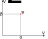
\includegraphics{images/diracPlot}
			\caption{Visual representation of Equation \ref{eq:ketNotationGeneric}. Vectors $V_1$ and $V_2$ must be orthogonal and normalized. $\alpha$ and $\beta$ represent the probabilities associated with the state $\psi$.}
			\label{fig:diracPlot2}
		\end{figure}
		
		\par When measured, a qubit will collapse to one of the basis states, either 1 or 0, with probabilities given by the magnitudes of $\alpha$ and $\beta$. Note the word \textbf{probability}, in this scope it means that due to \textbf{Heisenberg Principle} is not possible to known exactly the position and velocity of particle at the same time!
		
		\subsection{Qubit capacity}
			\begin{itemize}
				\item 1 qubit = 2 bits
				\item 2 qubits = 4 bits
				\item 3 qubits = 8 bits (1 byte)
				\item 4 qubits = 16 bits
				\item 13 qubits = 8.192 bits (1kb)
				\item 23 qubits = 8.388.608 bits (1mb)
				\item 33 qubits = 8.589.934.592 bits (1gb)
				\item 43 qubits = 8.796.093.022.208 bits (1 terabyte)
				\item n qubits = $2^n$ bits
			\end{itemize}
		
	\section{Quantum Superposition}
		\par The superposition principle.

	\section{Quantum Entanglement}
	
	\section{Quantum operations}
		\label{sec:quantumOperations}
				
		\par The state vector can be subject to \textbf{quantum operations}, such as unitary transformations and measurements. These operations modify the state vector or extract information from it, allowing for the study of the system's properties and the prediction of measurement outcomes.
		
	\section{Examples}
	
	\section{Conclusion}
		\par Quantum mechanics provides a fascinating framework for understanding the behavior of matter and energy at the microscopic level. The concepts of superposition and entanglement, in particular, are crucial for the development of quantum computation. By leveraging these concepts, quantum computers have the potential to solve certain problems much more efficiently than classical computers. By familiarizing ourselves with the basic principles of quantum mechanics, computer scientists can effectively explore and harness the power of quantum computation.
	
	\bibliographystyle{plain}
	\bibliography{references.bib}
\end{document}